%% ============================================================
%%  HoneyIQ — Extensions Addendum Slides
%%  Traffic Realism, Escalation Tracking, and Dynamic Response
%%  Compile: pdflatex slides_extensions
%%
%%  Figures expected in ../latex/figures/
%%  Standalone deck — does not modify slides.tex.
%% ============================================================
\documentclass[aspectratio=169, 12pt]{beamer}

%% ── Theme ────────────────────────────────────────────────────
\usetheme{Madrid}
\usecolortheme{seahorse}
\setbeamertemplate{navigation symbols}{}
\setbeamertemplate{footline}[frame number]

%% ── Packages ─────────────────────────────────────────────────
\usepackage[utf8]{inputenc}
\usepackage[T1]{fontenc}
\usepackage{lmodern}
\usepackage{graphicx}
\graphicspath{{../latex/figures/}{figures/}}
\usepackage{booktabs}
\usepackage{multirow}
\usepackage{amsmath, amssymb}
\usepackage{xcolor}
\usepackage{tikz}
\usetikzlibrary{arrows.meta, positioning, shapes.geometric}

%% ── Colours (matches slides.tex) ────────────────────────────
\definecolor{honeyblue}{RGB}{0,70,127}
\definecolor{honeyorange}{RGB}{220,100,30}
\definecolor{honeygrey}{RGB}{80,80,80}
\definecolor{alertred}{RGB}{180,30,30}
\definecolor{safegreen}{RGB}{30,130,80}

\setbeamercolor{title}{fg=white, bg=honeyblue}
\setbeamercolor{frametitle}{fg=white, bg=honeyblue}
\setbeamercolor{block title}{fg=white, bg=honeyblue}
\setbeamercolor{block title alerted}{fg=white, bg=alertred}
\setbeamercolor{block title example}{fg=white, bg=safegreen}

%% ── Metadata ─────────────────────────────────────────────────
\title[HoneyIQ Extensions]{%
  \textbf{HoneyIQ — Extensions}\\
  \large Traffic Realism, Escalation Tracking,\\ and Dynamic Response}
\subtitle{Addendum to the MSc Dissertation Presentation}
\author{G.W.P.\ Chamikara \\ \small Student ID: 239149P}
\institute{%
  Department of Computer Science \& Engineering\\
  Faculty of Engineering}
\date{August 2026}

%% ============================================================
\begin{document}

%% ── Title ────────────────────────────────────────────────────
\begin{frame}
  \titlepage
\end{frame}

\begin{frame}{Overview}
  \tableofcontents
\end{frame}

%% ============================================================
\section{What Was Still Missing}

\begin{frame}{Three Practical Gaps in the Original SEDM}
  \begin{columns}[T]
    \begin{column}{0.48\textwidth}
      \begin{alertblock}{1. Synthetic traffic was too uniform}
        Every network feature resampled independently, every step.
        No session had a consistent ``character.'' All benign traffic
        looked identical.
      \end{alertblock}
      \vspace{0.2cm}
      \begin{alertblock}{2. Escalation tracking was blunt}
        A hard 20-step sliding window, binary attack/no-attack —
        discards \emph{how bad} recent attacks were, not just how many.
      \end{alertblock}
    \end{column}
    \begin{column}{0.48\textwidth}
      \begin{alertblock}{3. Nothing was dynamic}
        Static thresholds, static matrix. No memory of a source IP
        across sessions. No response to sustained observed patterns.
      \end{alertblock}
      \vspace{0.2cm}
      \begin{exampleblock}{The open question}
        Would a learning-based approach (DQN) be a more practical way
        to close gap \#3? We already have data on that — see the end
        of this deck.
      \end{exampleblock}
    \end{column}
  \end{columns}
\end{frame}

%% ============================================================
\section{Realistic Synthetic Traffic}

\begin{frame}{Session-Coherent Traffic Instead of Per-Step Noise}
  \begin{center}
    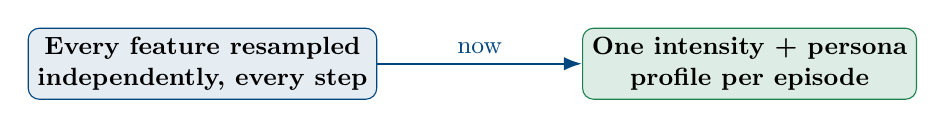
\begin{tikzpicture}[
        node distance=1.1cm,
        box/.style={rectangle, rounded corners, draw=honeyblue, fill=honeyblue!10,
                    minimum width=3.4cm, minimum height=0.9cm, align=center,
                    font=\small\bfseries},
      ]
      \node[box] (before) {Every feature resampled\\independently, every step};
      \node[box, right=2.6cm of before, fill=safegreen!15, draw=safegreen] (after)
        {One intensity + persona\\profile per episode};
      \draw[-Latex, thick, honeyblue] (before) -- node[above, font=\small] {now} (after);
    \end{tikzpicture}
  \end{center}
  \vspace{0.3cm}
  \begin{columns}[T]
    \begin{column}{0.48\textwidth}
      \begin{block}{Session intensity}
        $\iota \sim \text{Lognormal}(0, 0.35)$, applied to 8
        volume-shaped features (bytes, load, packet counts).
        TTL/window/duration untouched.
      \end{block}
    \end{column}
    \begin{column}{0.48\textwidth}
      \begin{block}{Three benign personas}
        \texttt{casual\_user} (70\%), \texttt{crawler} (20\%),
        \texttt{monitoring\_probe} (10\%) — instead of one fixed
        ``NORMAL'' distribution.
      \end{block}
    \end{column}
  \end{columns}
  \vspace{0.2cm}
  \begin{center}
    \textcolor{honeygrey}{\small Classifier training data regenerated with fresh
    intensity/persona per sample — retrained model: \textbf{99.4\% holdout accuracy}.}
  \end{center}
\end{frame}

%% ============================================================
\section{Better Escalation Tracking}

\begin{frame}{From a Hard Window to a Severity-Weighted EMA}
  \begin{columns}[T]
    \begin{column}{0.48\textwidth}
      \begin{block}{Before: sliding window}
        \[
          \rho_{\text{window}} = \frac{1}{|W|}\sum_{i \in W} \mathbb{1}[\text{attack}_i]
        \]
        \begin{itemize}
          \item Binary per step
          \item Hard cutoff at the window edge
          \item Recon probe = worm outbreak
        \end{itemize}
      \end{block}
    \end{column}
    \begin{column}{0.48\textwidth}
      \begin{exampleblock}{New: severity-weighted EMA}
        \[
          \rho^{(t)}_{\text{ema}} = \alpha\, s(\text{attack}_t) + (1-\alpha)\,\rho^{(t-1)}_{\text{ema}}
        \]
        \begin{itemize}
          \item Uses existing severity weights
          \item Smooth decay, no hard cutoff
          \item $\alpha = 0.15$
        \end{itemize}
      \end{exampleblock}
    \end{column}
  \end{columns}
  \vspace{0.3cm}
  \begin{alertblock}{Both signals always computed — opt-in, not a replacement}
    \texttt{escalation\_mode="window"} stays the default everywhere.
    \texttt{RATE\_THRESHOLD} was calibrated against window semantics, so
    EMA mode needs its own validation pass before relying on R3's
    trigger behaviour.
  \end{alertblock}
\end{frame}

%% ============================================================
\section{Dynamic Response}

\begin{frame}{Cross-Session Reputation: A New R4 Override}
  \begin{columns}[T]
    \begin{column}{0.52\textwidth}
      \begin{block}{The gap}
        Session state expires with its TTL (300s). A source IP that
        attacks, goes quiet, and comes back looks brand new.
      \end{block}
      \vspace{0.2cm}
      \begin{exampleblock}{ReputationTracker}
        Half-life-decayed offense score, per source IP, independent of
        individual sessions:
        \[
          \text{score}(t) = \text{score}(t_0)\cdot 0.5^{(t-t_0)/h}
        \]
        Default half-life: 6 hours.
      \end{exampleblock}
    \end{column}
    \begin{column}{0.44\textwidth}
      \begin{alertblock}{R4 — checked before R1}
        Reputation $\geq 0.60 \Rightarrow$ upgrade one severity level,
        \textbf{even on a benign-looking event}.
      \end{alertblock}
      \vspace{0.2cm}
      \begin{center}
        \small\textcolor{honeygrey}{Fail2ban-style: once flagged,\\ stay flagged.\\[4pt]
        Trade-off: a shared/dynamic IP\\ that was briefly malicious\\
        stays penalised for the\\ decay half-life.}
      \end{center}
    \end{column}
  \end{columns}
\end{frame}

\begin{frame}{Bounded Threshold Adaptation — Honestly Scoped}
  \begin{alertblock}{What we did \emph{not} build}
    \texttt{ESC\_LOW\_THRESHOLD} / \texttt{ESC\_HIGH\_THRESHOLD} adapt to
    \emph{nothing} — they bucket a risk computed purely from a static
    Markov model. No live signal exists to tune them against, so we
    didn't pretend otherwise.
  \end{alertblock}
  \vspace{0.3cm}
  \begin{columns}[T]
    \begin{column}{0.48\textwidth}
      \begin{block}{What we did build}
        \texttt{AdaptiveThresholds}: a bounded deadband controller that
        nudges \texttt{RATE\_THRESHOLD} to keep R3's firing rate near a
        target — an \textbf{alert-fatigue safety valve}, not a
        correctness fix.
      \end{block}
    \end{column}
    \begin{column}{0.48\textwidth}
      \begin{exampleblock}{Why the honesty matters}
        The only signal available is R3's \emph{own} trigger frequency
        — not whether any trigger was right. There's no ground-truth
        feedback loop in this system. Framing this as ``learning
        correctness'' would be dishonest.
      \end{exampleblock}
    \end{column}
  \end{columns}
  \vspace{0.2cm}
  \begin{center}
    \textcolor{honeyblue}{\small Verified: 60 sustained high-rate decisions moved the
    threshold toward its bound and stayed within it.}
  \end{center}
\end{frame}

%% ============================================================
\section{Is a Learning-Based Approach More Practical?}

\begin{frame}{Revisiting DQN — With Evidence We Already Have}
  \begin{columns}[T]
    \begin{column}{0.48\textwidth}
      \begin{alertblock}{What actually happened last time}
        \begin{itemize}
          \item Detection rate 87.6\% $\to$ 97.4\% in \emph{one episode}
          \item FPR pinned near \textbf{1.0} the whole time
          \item Learned ``almost never ALLOW,'' not real discrimination
          \item Trained on one intent only — wouldn't generalise
        \end{itemize}
      \end{alertblock}
    \end{column}
    \begin{column}{0.48\textwidth}
      \begin{alertblock}{Why the eval harness makes this worse}
        Two independent, hard-to-catch label-alignment bugs inflated
        measured FPR by up to $10\times$ before being caught — in code
        that only computed statistics \emph{after the fact}. A reward
        signal shapes learning on \emph{every step}.
      \end{alertblock}
    \end{column}
  \end{columns}
  \vspace{0.4cm}
  \begin{center}
    \large\textcolor{honeyblue}{\textbf{Conclusion: not practical right now.}
    The reputation override and the scoped threshold controller meet the
    same bar (Rudin, 2019) with none of the risk.}
  \end{center}
\end{frame}

\begin{frame}{If a Learning Component Is Ever Wanted}
  \begin{block}{Not a Q-network}
    A \textbf{small contextual bandit} choosing among 3--5 preset
    \texttt{RATE\_THRESHOLD} values — nothing more ambitious than that.
  \end{block}
  \vspace{0.3cm}
  \begin{exampleblock}{The one prerequisite that doesn't exist yet}
    A reward needs a \textbf{trustworthy signal}: an analyst's own
    confirmed true/false-positive label on a logged decision. Decisions
    are already logged in full — but nothing closes the loop from
    ``a human confirmed this was wrong'' back into a trainable signal.
  \end{exampleblock}
  \vspace{0.3cm}
  \begin{alertblock}{What we won't do}
    Manufacture a proxy signal (R1/R3 trigger rates) that \emph{looks}
    like learning without being grounded in ground truth — that's the
    same trap the original DQN fell into.
  \end{alertblock}
\end{frame}

%% ============================================================
\section{Summary}

\begin{frame}{Six Extensions, All Additive}
  \begin{center}
    \small
    \begin{tabular}{p{4.2cm}p{5.4cm}p{2.4cm}}
      \toprule
      \textbf{Extension} & \textbf{Mechanism} & \textbf{Default} \\
      \midrule
      Session-coherent traffic & Per-episode intensity/persona & Always on \\
      Benign traffic diversity & Three weighted personas & Always on \\
      Randomised event payloads & Wordlist/jitter resolution & Always on \\
      Escalation tracking & Severity-weighted EMA & Opt-in \\
      Cross-session reputation & Half-life decay + R4 & Tracked; R4 opt-triggered \\
      Threshold adaptation & Bounded deadband controller & Opt-in \\
      \bottomrule
    \end{tabular}
  \end{center}
  \vspace{0.4cm}
  \begin{center}
    \large\textcolor{honeyblue}{\textbf{Every new parameter defaults to the prior exact
    behaviour — nothing breaks by standing still.}}
  \end{center}
\end{frame}

\begin{frame}[plain]
  \begin{center}
    \vspace{1.5cm}
    {\Huge\textbf{Thank You}}\\[1cm]
    {\large HoneyIQ Extensions: Traffic Realism, Escalation Tracking,\\
    and Dynamic Response}\\[1cm]
    \begin{tabular}{rl}
      \textbf{Author:}     & G.W.P.\ Chamikara (239149P) \\
      \textbf{Supervisor:} & Dr.\ Thanuja Ambegoda \\
      \textbf{Degree:}     & MSc Data Science \& AI \\
      \textbf{Date:}       & August 2026 \\
    \end{tabular}\\[1cm]
    {\large\textit{Questions?}}
  \end{center}
\end{frame}

\end{document}
